\documentclass[11pt]{article}
\usepackage{../../tex/math-cmds}
\usepackage{../../tex/analysis}
\usepackage{mathabx}

   
\title{Lecture Notes:
		Advanced Interprocedural Analysis: Pointer Analysis and Object-Oriented Call Graph Construction}
\author{17-355/17-665/17-819: Program Analysis (Spring 2020)\\
        Claire Le Goues\footnote{These notes were developed together with Jonathan Aldrich}\\
		{\tt clegoues@cs.cmu.edu}}
\date{}

\begin{document}

\maketitle

We have successfully extended our interprocedural dataflow analysis framework to
a small functional programming language, which required us to reason explicitly
about which functions might be called, where. This provides insight into similar
problems in other programming paradigms, namely \emph{dynamic dispatch}.
Precisely addressing dynamic dispatch relies on techniques for \emph{pointer
  analysis}, which establishes which pointers can point to which locations.
Analyses that address real programming languages (whether they use dynamic
dispatch or not) must address pointers, because ignoring them dramatically
impacts analysis precision. Thus, in the interest of adapting our framework to
real languages, we turn our attention to these issues.

\section{Pointer Analysis}

\emph{Pointers} are variables whose value refers to another value elsewhere in
memory, by storing the address of that stored value. To illustrate why they
matter in analyzing real programs, consider constant-propagation analysis of the
following program:

\[
\begin{array}{ll}
1: & z := 1\\
2: & p := \&z\\
3: & *p := 2\\
4: & \mbox{print}~ z\\
\end{array}
\]

\noindent To analyze this program correctly we must be aware that at instruction 3, $p$ points to $z$.  If this information is available we can use it in a flow function as follows:

\[
\begin{array}{ll}

f_{CP}\parg{*p := y}(\sigma) & = \sigma[z \mapsto \sigma(y) ~|~ z \in \textit{must-point-to}(p)]\\[1ex]

\end{array}
\]

When we know exactly what a variable $x$ points to, we have \textit{must-point-to} information, and we can perform a \textit{strong update} of the target variable $z$, because we know with confidence that assigning to $*p$ assigns to $z$.  A technicality in the rule is quantifying over all $z$ such that $p$ must point to $z$.  How is this possible?  It is not possible in C or Java; however, in a language with pass-by-reference, for example C++, it is possible that two names for the same location are in scope.

Of course, it is also possible to be uncertain to which of several distinct locations $p$ points:

\[
\begin{array}{ll}
1: & z := 1\\
2: & \mathbf{if}~ (\textit{cond})~ p := \&y ~\mathbf{else}~ p := \&z\\
3: & *p := 2\\
4: & \mathbf{print}~ z\\
\end{array}
\]

Now constant propagation analysis must conservatively assume that $z$ could hold either 1 or 2.  We can represent this with a flow function that uses may-point-to information:

\[
\begin{array}{ll}

f_{CP}\parg{*p := y}(\sigma) & = \sigma[z \mapsto \sigma(z) \join \sigma(y) ~|~ z \in \textit{may-point-to}(p)]\\[1ex]

\end{array}
\]

\todo{Consider starting with an analysis that's flow-sensitive?  But that would take more than one lecture, most likely}

\subsection{Andersen's Points-To Analysis}

Two common kinds of pointer analysis are \emph{alias analysis} and
\emph{points-to} analysis. Alias analysis computes sets $S$ holding pairs of
variables $(p,q)$, where $p$ and $q$ may (or must) point to the same location.
Points-to analysis computes the set $\textit{points-to}(p)$, for each pointer
variable $p$, where the set contains a variable $x$ if $p$ may (or must) point
to the location of the variable $x$. We will focus primarily on points-to
analysis, beginning with a simple but useful approach originally proposed by
Andersen.\footnote{PhD thesis: ``Program Analysis and Specialization for the C
Programming Language.''}

Our initial setting will be C programs. We are interested in analyzing
instructions that are relevant to pointers in the program. Ignoring for the
moment memory allocation and arrays, we can decompose all pointer operations in
C into four types:

\[
\begin{array}{llll}
I & \bnfdef & ... \\
  & \bnfalt & p := \&x & \mbox{taking the address of a variable} \\
  & \bnfalt & p := q & \mbox{copying a pointer from one variable to another}\\
  & \bnfalt & *p := q & \mbox{assigning through a pointer}\\
  & \bnfalt & p := *q & \mbox{dereferencing a pointer} \\
\end{array}
\]

Andersen's points-to analysis is a context-insensitive interprocedural analysis.
It is also a \textit{flow-insensitive analysis}, that is an analysis that does
not consider program statement order. Context- and flow-insensitivity improve
analysis performance, as precise pointer analysis can be notoriously expensive.

We will formulate Andersen's analysis by generating set constraints which can
later be processed by a set constraint solver, much like we did for CFA. Because
the analysis is flow-insensitive, we do not care what order the instructions in
the program come in; we simply generate a set of constraints and solve them.
Constraint generation for each statement works by these rules: 

\[
\begin{array}{c}
\infer[\textit{address-of}]
	{\parg{p := \&x} \hookrightarrow l_x \in p}
	{}\\[3ex]
	
\infer[\textit{copy}]
	{\parg{p := q} \hookrightarrow p \supseteq q}
	{}\\[3ex]
	
\infer[\textit{assign}]
	{\parg{*p := q} \hookrightarrow *p \supseteq q}
	{}\\[3ex]
	
\infer[\textit{dereference}]
	{\parg{p := *q} \hookrightarrow p \supseteq *q}
	{}\\[3ex]
	
\end{array}
\]

The first rule states that a constant location $l_x$, representation the address
of $x$, is in the set of location pointed to by $p$. The second rule states that
the set of locations pointed to by $p$ must be a superset of those pointed to by
$q$. The last two rules state the same, but take into account that one or the
other pointer is dereferenced. Note that if Andersen's algorithm says that the
set $p$ points to only one location $l_z$, we have \emph{must-point-to}
information, whereas if the set $p$ contains more than one location, we have
only \emph{may-point-to} information.

A number of specialized set constraint solvers exist, and constraints in the
form above can be translated into input for them.\footnote{Note that the
  dereference operation (the $*$ in $*p \supseteq q$) is not standard, but can
  be encoded,} We will treat constraint-solving abstractly using the following
constraint propagation rules:

% COME UP WITH THESE BY EXAMPLE IN CLASS

\[
\begin{array}{c}
\infer[\textit{copy}]
	{l_x \in p}
	{p \supseteq q & l_x \in q}\\[3ex]
		
\infer[\textit{assign}]
	{l_x \in r}
	{*p \supseteq q & l_r \in p & l_x \in q}\\[3ex]
	
\infer[\textit{dereference}]
	{l_x \in p}
	{p \supseteq *q & l_r \in q & l_x \in r}\\[3ex]
	
\end{array}
\]

\todo{come up with pictures, with dotted lines for the added edge}

\todo{which programs above in particular?  Better to get an interesting example that uses all Andersen rules}

We can now apply Andersen's points-to analysis to the programs above. 
%
We can also apply it to programs with dynamic memory allocation, such as:

\[
\begin{array}{ll}
1: & q := \textit{malloc}()\\
2: & p := \textit{malloc}()\\
3: & p := q\\
4: & r := \&p\\
5: & s := \textit{malloc}()\\
6: & *r := s\\
7: & t := \&s\\
8: & u := *t\\
\end{array}
\]

The analysis is run the same way, but we treat the memory cell allocated at each
\textit{malloc} or \textit{new} statement as an abstract location labeled by the
location $n$ of the allocation point:

\[
\begin{array}{c}
\infer[\textit{malloc}]
	{\parg{n{:}~ p := \textit{malloc}()} \hookrightarrow l_n \in p}
	{}\\[3ex]
	
\end{array}
\]

We must be careful because a \textit{malloc} statement can be executed more than
once, and each time it executes, a new memory cell is allocated. Unless we have
some other means of proving that the malloc executes only once, we must assume
that if some variable $p$ only points to one abstract malloc'd location $l_n$,
that is still may-alias information (i.e. $p$ points to only one of the many
actual cells allocated at the given program location) and not must-alias
information.

\paragraph{Efficiency.} Analyzing the efficiency of Andersen's algorithm, we can see that all
constraints can be generated in a linear $O(n)$ pass over the program. The
solution size is $O(n^2)$, because each of the $O(n)$ variables defined in the
program could potentially point to $O(n)$ other variables.

We can derive the execution time as follows:\footnote{David A. McAllester. 1999.
  On the Complexity Analysis of Static Analyses. In Proceedings of the 6th
  International Symposium on Static Analysis (SAS ’99): 312–329.} There are
$O(n)$ flow constraints generated of the form $p \supseteq q$, $*p \supseteq q$,
or $p \supseteq *q$. How many times could a constraint propagation rule fire for
each flow constraint? For a $p \supseteq q$ constraint, the rule may fire at
most $O(n)$ times, because there are at most $O(n)$ premises of the proper form
$l_x \in p$. However, a constraint of the form $p \supseteq *q$ could cause
$O(n^2)$ rule firings, because there are $O(n)$ premises each of the form
$l_x \in p$ and $l_r \in q$. With $O(n)$ constraints of the form
$p \supseteq *q$ and $O(n^2)$ firings for each, we have $O(n^3)$ constraint
firings overall. A similar analysis applies for $*p \supseteq q$ constraints.
McAllester's theorem states that the analysis with $O(n^3)$ rule firings can be
implemented in $O(n^3)$ time. Thus we have derived that Andersen's algorithm is
cubic in the size of the program, in the worst case.

Interestingly, Andersen's algorithm can be executed in $O(n^2)$ time for
\textit{k-sparse} programs.\footnote{Manu Sridharan and Stephen J. Fink. 2009.
  The Complexity of Andersen’s Analysis in Practice. In Proceedings of the 16th
  International Symposium on Static Analysis (SAS ’09): 205–221.} The
\textit{k-sparse} assumption requires that at most $k$ statements dereference
each variable, and that the flow graph is sparse. The publication showing this
result also showed that typical Java programs are \textit{k-sparse}, and that
Andersen's algorithm scales quadratically in practice.

\subsection{Field Sensitivity}

What happens when we have a pointer to a struct in C, or an object in an
object-oriented language? In this case, we would like the pointer analysis to
tell us what each field in the struct or object points to. A simple solution is
to be \textit{field-insensitive}, treating all fields in a struct as equivalent.
Thus if $p$ points to a struct with two fields $f$ and $g$, and we assign:

\[
\begin{array}{ll}
1: & p.f := \&x\\
2: & p.g := \&y\\
\end{array}
\]

A field-insensitive analysis would tell us (imprecisely) that $p.f$ could point
to $y$. We can modify the rules above by treating any field dereference or field
assignment to $p.f$ as a pointer dereference $*p$. Essentially, you can think of
this as just considering all fields to be named $*$.

To be more precise, we can instead track the contents each field of each abstract
location separately. In the discussion below, we assume a Java-like setting, in
which all objects are allocated on the heap and where we cannot take the address
of a field. A slightly more complicated variant of this scheme works in C-like
languages.

We will use the \textit{malloc} and \textit{copy} rules unchanged from
above.\footnote{In Java, the \texttt{\textbf{new}} expression plays the role of
  \texttt{malloc}} We drop the \textit{assign} and \textit{dereference} rules,
and replace them with: 

\[
\begin{array}{c}
\infer[\textit{field-read}]
	{\parg{p := q.f} \hookrightarrow p \supseteq q.f}
	{}\\[3ex]
	
\infer[\textit{field-assign}]
	{\parg{p.f := q} \hookrightarrow p.f \supseteq q}
	{}\\[3ex]
	
\end{array}
\]


Now assume that objects (e.g. in Java) are represented by abstract locations
$l$. We will have two forms of basic facts. The first is the same as before:
$l_n \in p$, where $l_n$ is an object allocated in a \texttt{\textbf{new}}
statement at line $n$. The second basic fact is $l_n \in l_m.f$, which states
that the field $f$ of the object represented by $l_m$ may point to an object
represented by $l_n$.

We can now process field constraints with the following rules:

\[
\begin{array}{c}
\infer[\textit{field-read}]
	{l_f \in p}
	{p \supseteq q.f & l_q \in q & l_f \in l_q.f}\\[3ex]
	
\infer[\textit{field-assign}]
	{l_q \in l_p.f}
	{p.f \supseteq q & l_p \in p & l_q \in q}\\[3ex]
	
\end{array}
\]

If we run this analysis on the code above, we find that it can distinguish that
$p.f$ points to $x$ and $p.g$ points to $y$.


\subsection{Steensgaard's Points-To Analysis}

For very large programs, a quadratic-in-practice algorithm is too inefficient.
Steensgaard proposed an pointer analysis algorithm that operates in near-linear
time, supporting essentially unlimited practical scalability.

The first challenge in designing a near-linear time points-to analysis is to
represent the results in linear space. This is nontrivial because over the
course of program execution, any given pointer $p$ could potentially point to
the location of any other variable or pointer $q$. Representing all of these
pointers explicitly will inherently take $O(n^2)$ space.

The solution Steensgaard found is based on using constant space for each
variable in the program. His analysis associates each variable $p$ with an
abstract location named after the variable. Then, it tracks a single points-to
relation between that abstract location $p$ and another one $q$, to which it may
point. Now, it is possible that in some real program $p$ may point to both $q$
and some other variable $r$. In this situation, Steensgaard's algorithm
\textit{unifies} the abstract locations for $q$ and $r$, creating a single
abstract location representing both of them. Now we can track the fact that $p$
may point to either variable using a single points-to relationship.

For example, consider the program to the left, and the graph that Andersen's points-to analysis would produce (right):

\begin{center}
\begin{minipage}[t]{0.30\textwidth} % toggle vertical alignment of table
\vspace{-10em}
$\begin{array}{ll}
1: & p := \&x\\
2: & r := \&p\\
3: & q := \&y\\
4: & s := \&q\\
5: & r := s\\
\end{array}$
\end{minipage}
\hspace*{1em}
\begin{minipage}[b]{0.30\textwidth}
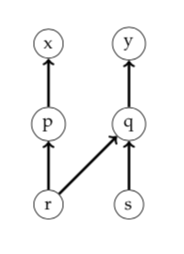
\includegraphics[scale=0.5]{images/andersens1}
\end{minipage}
\end{center}

%\begin{tikzpicture}[scale=1.75]
%\GraphInit[vstyle=Normal]
%\Vertex{x}
%\Vertex[x=0,y=-1]{p}
%\Vertex[x=0,y=-2]{r}
%\Vertex[x=1,y= 0]{y}
%\Vertex[x=1,y=-1]{q}
%\Vertex[x=1,y=-2]{s}
%\SetUpEdge[style={->,ultra thick}]
%\Edges(r,p,x)
%\Edges(s,q,y)
%\Edge(r)(q)
%\end{tikzpicture}

But in Steensgaard's setting, when we discover that $r$ could point both to $q$ and to $p$, we must merge $q$ and $p$ into a single node:
\begin{center}
\begin{tikzpicture}[scale=1.25]
\GraphInit[vstyle=Normal]
\Vertex{x}
\Vertex[x=0.5,y=-1]{pq}
\Vertex[x=0,y=-2]{r}
\Vertex[x=1,y= 0]{y}
\Vertex[x=1,y=-2]{s}
\SetUpEdge[style={->,ultra thick}]
\Edges(r,pq,x)
\Edges(s,pq,y)
\end{tikzpicture}
\end{center}

Notice that we have lost precision: by merging the nodes for $p$ and $q$ our graph now implies that $s$ could point to $p$, which is not the case in the actual program.  But we are not done.  Now $pq$ has two outgoing arrows, so we must merge nodes $x$ and $y$.  The final graph produced by Steensgaard's algorithm is therefore:

\begin{center}
\begin{tikzpicture}[scale=1.25]
\GraphInit[vstyle=Normal]
\Vertex{xy}
\Vertex[x=0,y=-1]{pq}
\Vertex[x=-0.5,y=-2]{r}
\Vertex[x=0.5,y=-2]{s}
\SetUpEdge[style={->,ultra thick}]
\Edges(r,pq,xy)
\Edges(s,pq)
\end{tikzpicture}
\end{center}

We study Steensgaard's analysis more precisely by specifying
a simplified version that ignores function pointers:

\[
\begin{array}{c}
\infer[\textit{copy}]
	{\parg{p := q} \hookrightarrow \textit{join}(*p,*q)}
	{}\\[3ex]
	
\infer[\textit{address-of}]
	{\parg{p := \&x} \hookrightarrow \textit{join}(*p,x)}
	{}\\[3ex]
	
\infer[\textit{dereference}]
	{\parg{p := *q} \hookrightarrow \textit{join}(*p,*{*}q)}
	{}\\[3ex]
	
\infer[\textit{assign}]
	{\parg{*p := q} \hookrightarrow \textit{join}(*{*}p,*q)}
	{}\\[3ex]
	
\end{array}
\]

With each abstract location $p$, we associate the abstract location that $p$
points to, denoted $*p$. Abstract locations are implemented as a
union-find\footnote{See any algorithms textbook} data structure so that we can
merge two abstract locations efficiently. In the rules above, we implicitly
invoke \textit{find} on an abstract location before calling \textit{join} on it,
or before looking up the location it points to.

The \textit{join} operation essentially implements a union operation on the
abstract locations. However, since we are tracking what each abstract location
points to, we must update this information also. The algorithm to do so is as
follows:

\lstdefinestyle{javastyle} {
language=Java,
basicstyle=\ttfamily\footnotesize,
  morekeywords={virtualinvoke},
  keywordstyle=\color{blue},
  ndkeywordstyle=\color{red},
  commentstyle=\color{dkred},
  stringstyle=\color{dkgreen},
  numbers=none,
  breaklines=true,
  numberstyle=\ttfamily\footnotesize\color{gray},
  stepnumber=1,
  numbersep=10pt,
  backgroundcolor=\color{white},
  tabsize=4,
  showspaces=false,
  showstringspaces=false,
  xleftmargin=.23in
}
\lstset{style=javastyle}

\begin{lstlisting}[mathescape]
join($\ell_1, \ell_2$)
    if (find($\ell_1$) == find($\ell_2$))
        return
    $n_1 \gets *\ell_1$
    $n_2 \gets *\ell_2$
    union($\ell_1, \ell_2$)
    join($n_1, n_2$)
\end{lstlisting}


Once again, we implicitly invoke \textit{find} on an abstract location before comparing it for equality, looking up the abstract location it points to, or calling \textit{join} recursively.

As an optimization, Steensgaard does not perform the join if the right hand side is not a pointer.  For example, if we have an assignment $\parg{p := q}$ and $q$ has not been assigned any pointer value so far in the analysis, we ignore the assignment.  If later we find that $q$ may hold a pointer, we must revisit the assignment to get a sound result.

Steensgaard illustrated his algorithm using the following program, and the graph
the algorithm produces:

\begin{center}
\begin{minipage}[t]{0.3\textwidth}
\vspace{-10em}
$\begin{array}{ll}
1: & a := \&x\\
2: & b := \&y\\
3: & \mbox{if}~ p ~\mbox{then}\\
4: & ~~~~ y := \&z\\
5: & \mbox{else}\\
6: & ~~~~ y := \&x\\
7: & c := \&y\\
\end{array}
$
\end{minipage}
\hspace*{1em}
\begin{minipage}[b]{0.30\textwidth}
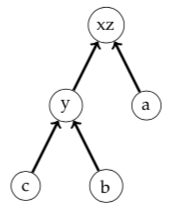
\includegraphics[scale=0.6]{images/steensgard1}
\end{minipage}
\end{center}

% \begin{tikzpicture}[scale=1.75]
% \GraphInit[vstyle=Normal]
% \Vertex{c}
% \Vertex[x=1,y=0]{b}
% \Vertex[x=0.5,y=1]{y}
% \Vertex[x=1.5,y=1]{a}
% \Vertex[x=1,y=2]{xz}
% \SetUpEdge[style={->,ultra thick}]
% \Edges(a,xz)
% \Edges(y,xz)
% \Edges(b,y)
% \Edges(c,y)
% \end{tikzpicture}
% 

%Rayside demonstrates the difference in precision between Andersen's and Steensgaard's analyses using the following program:

%\[
%\begin{array}{ll}
%1: & p := \textit{malloc}_1()\\
%2: & q := \textit{malloc}_2()\\
%3: & fp:= \&p\\
%4: & fp:= \&q\\
%5: & ... := *fp\\
%\end{array}
%\]


\paragraph{Efficiency.} Rayside illustrates how Andersen must sometimes do more work than
Steensgaard:

\todo{Cite Rayside notes}

\[
\begin{array}{ll}
1: & q := \&x\\
2: & q := \&y\\
3: & p := q\\
4: & q := \&z\\
\end{array}
\]

After processing the first three statements, Steensgaard's algorithm will have
unified variables $x$ and $y$, with $p$ and $q$ both pointing to the unified
node. Andersen's algorithm will have both $p$ and $q$ pointing to
both $x$ and $y$. When the fourth statement is processed, Steensgaard's
algorithm does only a constant amount of work, merging $z$ in with the
already-merged $xy$. On the other hand, Andersen's algorithm must not just
create a points-to relation from $q$ to $z$, but must also propagate that
relationship to $p$. It is this additional propagation step that results in the
significant performance difference between these algorithms.\footnote{For fun,
  try adding a new statement $r := p$ after statement 3. Then $z$ has to be
  propagated to the points-to sets of both p and r. In general, the number of
  propagations can be linear in the number of copies and the number of
  address-of operators, which makes it quadratic overall even for programs in
  the simple form above.}

Analyzing Steensgaard's pointer analysis for efficiency, we observe that each of
$n$ statements in the program is processed once. The processing is linear,
except for \textit{find} operations on the union-find data structure (which may
take amortized time $O(\alpha(n))$ each) and the \textit{join} operations. We
note that in the \textit{join} algorithm, the short-circuit test will fail at
most $O(n)$ times---at most once for each variable in the program. Each time the
short-circuit fails, two abstract locations are unified, at cost $O(\alpha(n))$.
The unification assures the short-circuit will not fail again for one of these
two variables. Because we have at most $O(n)$ operations and the amortized cost
of each operation is at most $O(\alpha(n))$, the overall running time of the
algorithm is near linear: $O(n * \alpha(n))$. Space consumption is linear, as no
space is used beyond that used to represent abstract locations for all the
variables in the program text.

Based on this asymptotic efficiency, Steensgaard's algorithm was run on a 1
million line program (Microsoft Word) in 1996; this was an order of magnitude
greater scalability than other pointer analyses known at the time.

Steensgaard's pointer analysis is field-insensitive; making it field-sensitive
would mean that it is no longer linear.

\section{Dynamic dispatch}

\emph{Dynamic dispatch} is the process of selecting which implementation of a
method or function should be called at runtime; it is a defining characteristic
object-oriented programming languages and systems, but is not limited to them
(e.g., calling through function pointers in C). To construct a precise call
graph in such languages, an analysis must determine the type of the receiver
object is at each call site. Flow analysis techniques similar to points-to
analysis can be used to compute this information, but using an interprocedural
flow analysis off the shelf requires a call graph, which is exactly what we are
trying to construct. Therefore, object-oriented call graph construction
algorithms must simultaneously build a call graph and compute dataflow
information describing the types of the objects to which each variable could
point.

\subsection{Simple approaches}

Before examining a full-fledged dataflow analysis-based call graph construction
algorithm, we will consider two simpler approaches that do not require flow
analysis. These approaches have the side benefit of being very efficient, and so
are used in settings such as JIT compilers where analysis time is scarce.

The simplest approach, \emph{class hierarchy analysis}, uses the type of a
variable, together with the class hierarchy, to determine what types of object
the variable could point to. Unsurprisingly, this is very imprecise, but can be
computed very efficiently in $O(n*t)$ time, because it visits $n$ call sites and
at each call site traverses a subtree of size $t$ of the class hierarchy.

An improvement to class hierarchy analysis is \textit{rapid type analysis},
which eliminates from the hierarchy classes that are never instantiated. The
analysis iteratively builds a set of instantiated types, method names invoked,
and concrete methods called. Initially, it assumes that \texttt{main} is the
only concrete method that is called, and that no objects are instantiated. It
then analyzes concrete methods known to be called, one by one. When a method name
is invoked, it is added to the list, and all concrete methods with that name
defined within (or inherited by) types known to be instantiated are added to the
called list. When an object is instantiated, its type is added to the list of
instantiated types, and all its concrete methods that have a method name that is
invoked are added to the called list. This proceeds iteratively until a fixed
point is reached, at which point the analysis knows all of the object types that
may actually be created at run time.

Rapid type analysis can be considerably more precise than class hierarchy
analysis in programs that use libraries that define many types, only a few of
which are used by the program. It remains extremely efficient, because it only
needs to traverse the program once (in $O(n)$ time) and then build the call
graph by visiting each of $n$ call sites and considering a subtree of size $t$
of the class hierarchy, for a total of $O(n*t)$ time.

\subsection{0-CFA Style Object-Oriented Call Graph Construction}

Object-oriented call graphs can also be constructed using a pointer analysis
such as Andersen's algorithm, either context-insensitive or context-sensitive.
The context-sensitive versions are called k-CFA by analogy with control-flow
analysis for functional programs. The context-insensitive version is called
0-CFA for the same reason. Essentially, the analysis proceeds as in Andersen's
algorithm, but the call graph is built up incrementally as the analysis
discovers the types of the objects to which each variable in the program can
point.

Even 0-CFA analysis can be considerably more precise than Rapid Type Analysis.
For example, in the program below, RTA would assume that any implementation of
foo() could be invoked at any program location, but 0-CFA can distinguish the
two call sites:

\begin{lstlisting}
class A { A foo(A x) { return x; } }
class B extends A { A foo(A x) { return new D(); } }
class D extends A { A foo(A x) { return new A(); } }
class C extends A { A foo(A x) { return this; } }

// in main()
A x = new A();
while (...)
    x = x.foo(new B()); // may call A.foo, B.foo, or D.foo
A y = new C();
y.foo(x);               // only calls C.foo
\end{lstlisting}

\end{document}
